\chapter{Fenómenos de superficie}	

\begin{miparrafo}
\begin{multicols}{2}
\small{Una diferencia fundamental entre gases y líquidos es la existencia de una superficie libre en éstos.}
\small{Gran variedad de fenómenos físicos están asociados a la existencia de esta superficie, y que se explican a partir de las propiedades contráctiles de ésta.}
\small{Este estado de tensión de la superficie libre del líquido tiende a reducir el área de ésta a un valor mínimo compatible con los vínculos y con las fuerzas externas. }
\begin{figure}[H]
	\centering
	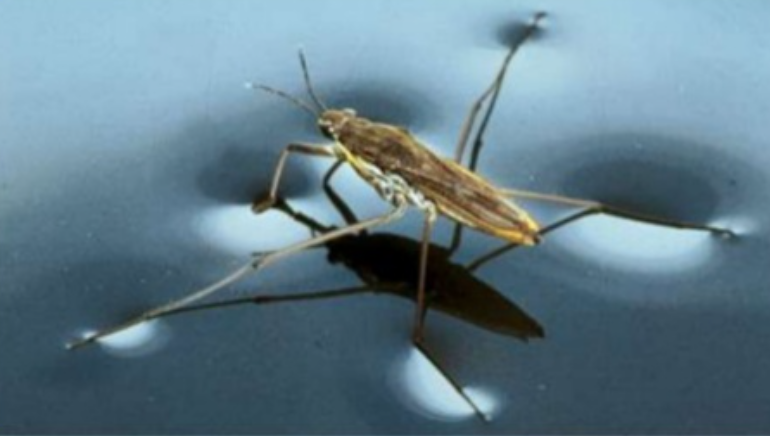
\includegraphics[width=.5\textwidth]{imagenes/imagenes08/T08IM01.png}
\end{figure}
\end{multicols}
 \small{1. Las gotas de lluvia o las burbujas de aire en el interior de un líquido tienden a tomar la forma que ofrece una superficie mínima, esférica. }
 
 \small{2. Una aguja de coser (a pesar de que su densidad es mayor que la del agua) o un insecto pueden flotar en el agua.}
 
 \small{3. Cuando sumergimos parcialmente en agua un tubo de vidrio, limpio y de pequeño calibre, el agua asciende en su interior, pero si lo sumergimos en mercurio, el líquido desciende}\normalsize{.}

\end{miparrafo}
	
\section{Tensión superficial}
	
\normalsize{Para} realizar un estudio macroscópico del comportamiento de la superficie límite de un líquido vamos a ver el comportamiento microscópico de una molécula	 y después, sumando contribuciones de muchas moléculas, pasaremos al punto de vista macroscópico.

Experimentalmente sabemos que las fuerzas que mantienen unidas a las moléculas o átomos son de naturaleza eléctrica, atractivas, que se establecen entre las cortezas electrónicas de los átomos y los núcleos atómicos (positivos) de los átomos vecinos. Estas fuerzas se conocen con el nombre de \emph{fuerzas de Van der Waals}, su intensidad es muchísimo mayor a la de la interacción gravitatoria y son de \emph{corto alcance}, tienen gran intensidad para distancias cortas (del orden de unos cuantos diámetros atómicos) pero decaen rápidamente al aumentar la distancia.

Podemos distinguir dos tipos de \emph{fuerzas de Van der Waals:}
\begin{itemize}
\vspace{-2mm} \item \emph{Fuerzas de cohesión:} son fuerzas de Van der Waals que se ejercen entre moléculas de una misma sustancia (agua-agua).
\vspace{-2mm} \item \emph{Fuerzas de adhesión:} son fuerzas de Van der Waals que se ejercen entre moléculas de sustancias distintas (agua-vaso).	
\end{itemize}
Las moléculas en el líquido están sometidas a las fuerzas de Van der Waals de corto alcance.
\begin{multicols}{2}
En el interior del fluido, por simetría, estas fuerzas se anulan.

Sobres las moléculas situadas en la superficie (libre o límite) del líquido no ocurre lo mismo y existe una fuerza resultante que trata de meterlas hacia dentro.
\begin{figure}[H]
	\centering
	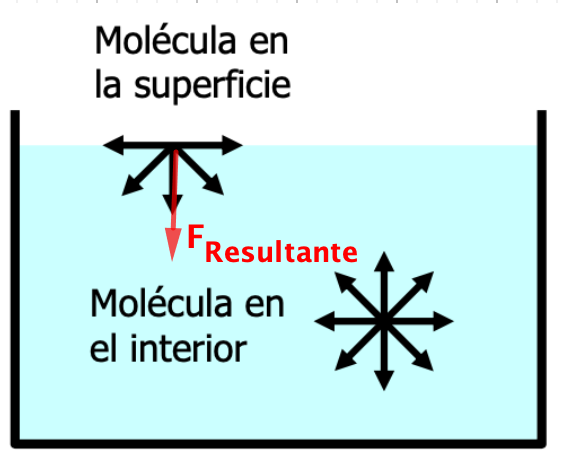
\includegraphics[width=.4\textwidth]{imagenes/imagenes08/T08IM02.png}
\end{figure}
\end{multicols}
Supongamos que sacamos a una de estas moléculas desde el interior a la superficie libre del líquido, tendremos que realizar un trabajo contra la resultante de la fuerza de la que hemos hablado anteriormente. Como los campos que generan las fuerzas de Van der Waals son conservativos, este trabajo vendrá de una diferencia de energías potenciales. Cuantas más moléculas subamos mayor será la superficie y más energía potencial tendremos: a mayor $\mathcal E_p$, mayor superficie $S$.

Teniendo en cuenta el teorema de Lejeune-Dirichlet, para que la molécula que subimos a la superficie ocupe una posición de equilibrios estable debe tener energía potencial mínima. Como la superficie mínima más estable es la esfera, ello explica por qué \emph{las gotas son esféricas}.

Cada vez que se modifica la superficie libre de un líquido una cantidad $\dd S$ hay que realizar un trabajo $\dd W$ que será proporcional ($\sigma=$constante de proporcionalidad)al cambio en la superficie:$ \subrayado{\ \boldsymbol{\dd W=\sigma \ \dd S\ }}$.

Esta constante de proporcionalidad, $\ \boldsymbol{\sigma} \ $, recibe el nombre de \emph{\textbf{coeficiente de tensión superficial}} y su valor depende de las propiedades físico-químicas del líquido del que se trate.


Unidades y dimensiones del coeficiente de tensión superficial:

$[\sigma]=\dfrac {[\mathrm{W}]}{[\mathrm{S}]}=\dfrac {[\mathrm{FL}]}{[\mathrm{S}]}=\mathrm{M}T^{-2}$; $\quad$ unidad SI: $\mathrm{J\ m}^{-2}$.


\emph{El coeficiente de tensión superficial es debido a fuerzas de cohesión}.
\begin{itemize}
\item No se manifiesta en los sólidos debido a la propia rigidez de éstos, a su incapacidad de movimiento.
\item No se manifiesta en los gases pues la moléculas del gas están a gran distancia unas de otras y las fuerzas de cohesión son de corto alcance.	
\end{itemize}

\subsection{Otra forma de introducir la tensión superficial}

Ésta, basada en la experiencia. 

En la figura, al tirar del alambre se observa cierta resistencia a la separación (fuerza), si se suelta vuelve a su posición inicial. Este fenómeno es debido a la tensión superficial.

Para cuantificar esta fuerza (de cohesión) consideremos una estructura de alambre con un lado deslizante, en la que se coloca una capa de líquido (solución jabonosa).
 
El líquido tratará de minimizar la superficie S ejerciendo una fuerza F sobre el lado deslizante, que S podemos medir. Se observa que: 
\begin{multicols}{2}

--- La tensión superficial $\sigma$ es la fuerza por unidad de longitud que ejerce la superficie de un líquido sobre una línea cualquiera situada sobre ella (borde de sujeción).

--- La fuerza debida a la tensión superficial es perpendicular a la línea y tangente a la superficie. 

\begin{figure}[H]
	\centering
	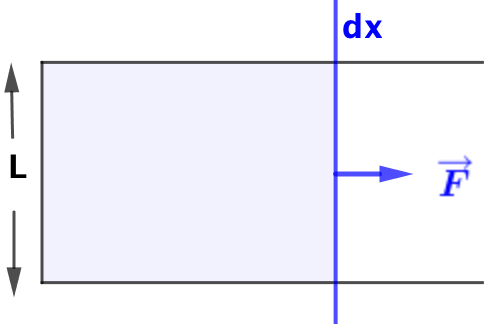
\includegraphics[width=.5\textwidth]{imagenes/imagenes08/T08IM03.png}
\end{figure}
\end{multicols}

\vspace{-3mm}La explicación física de este fenómeno es la siguiente:

Al estirar, aumentamos la superficie con lo que, según hemos visto, aumenta la energía potencial y se realiza un trabajo: $\ \dd W=F_T \dd x$, puesto que la película de solución jabonosa (fluido) se extiende por arriba y por abajo (un líquido en un vaso solo tiene una), el trabajo en deformar la superficie es: $\ \dd W=\sigma \dd S=\sigma 2L \dd x$, por lo que $F_T=2\sigma L=2F$, una para la superficie de arriba y otra para la de abajo. 

Se deduce: $\subrayado{\ \sigma=\dfrac F L \ }$, fuerza que actúa sobre la unidad de longitud sobre la superficie libre de un líquido. Esta es la causa por la que se llama \emph{tensión} superficial.
\begin{multicols}{2}
\footnotesize{El peso del insecto queda compensado por la resistencia de la superficie del agua a ser deformada. Esta fuerza sólo tiene componente vertical, pues la horizontal se anula.}
\footnotesize{$F_y=2\pi r \sigma \cos \theta \ n$, que compensará al peso del insecto. $\sigma$ es la tensión superficial, $r$ el radio de la depresión que producen las patas y $n$ el número de patas}\normalsize{.}
\begin{figure}[H]
	\centering
	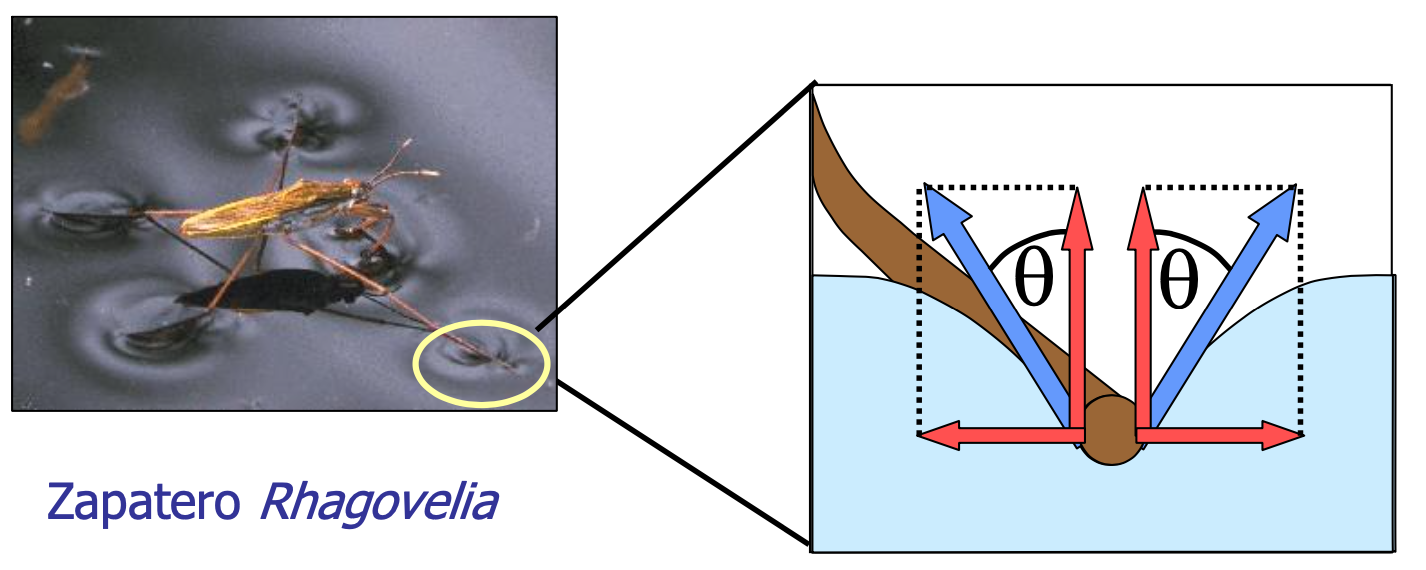
\includegraphics[width=.5\textwidth]{imagenes/imagenes08/T08IM19.png}
\end{figure}
\end{multicols}

\section{Superficie de contacto. Meniscos}
Debido a la interacción que se ejerce entre el líquido y el recipiente que lo contiene (fuerzas de adhesión y cohesión de Van der Waals), la superficie libre del líquido deja de ser plana y adopta la forma que aparece en la figura. Este fenómeno recibe el nombre de \emph{menisco}.

Se llama \emph{ángulo de conjunción} o de contacto, $\theta$ al formado por la tangente a la superficie libre del líquido en el punto de contacto con el recipiente contenedor con la pared de éste último.
\vspace{-3mm} %***************************
\begin{figure}[H]
	\centering
	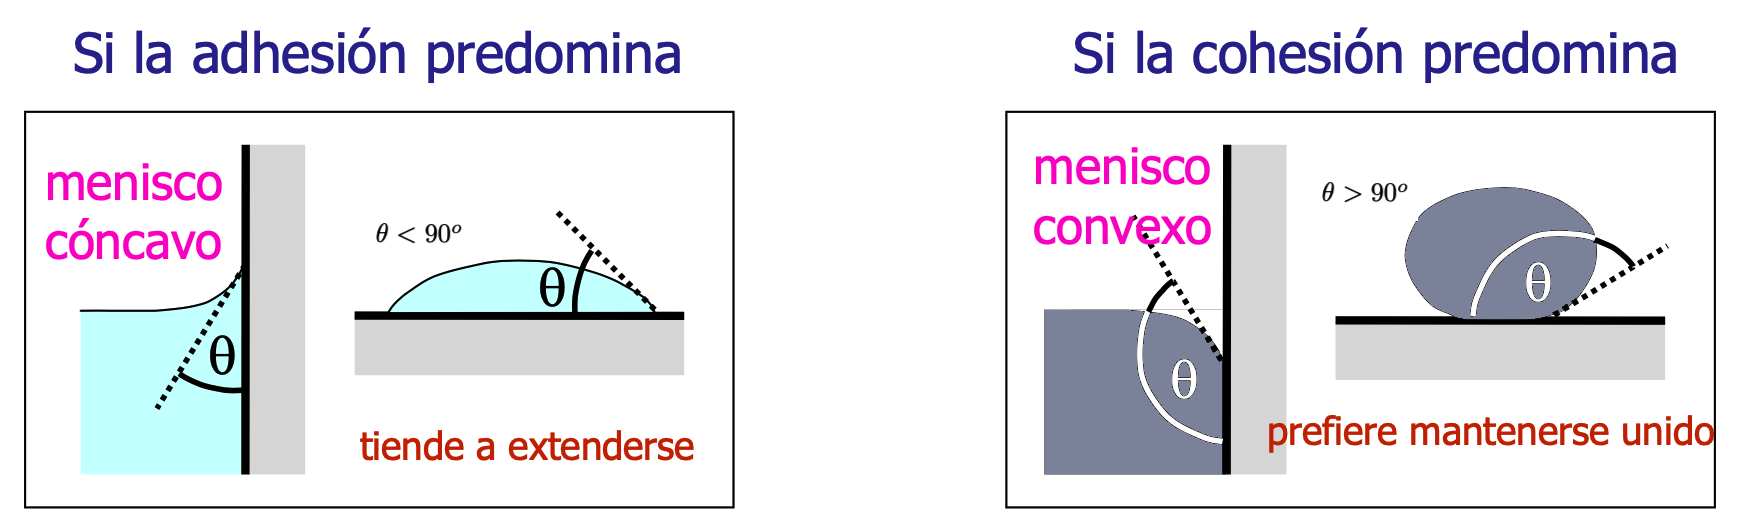
\includegraphics[width=.9\textwidth]{imagenes/imagenes08/T08IM04.png}
\end{figure}
\vspace{-3mm} %***************************
\begin{itemize}
\item Si el ángulo de conjunción es $\theta<90^0$ el menisco se llama \emph{cóncavo} y se dice que \emph{el líquido moja el vaso} (agua-vidrio).

\item Si el ángulo de conjunción es $\theta>90^0$ el menisco se llama \emph{convexo} y se dice que \emph{el líquido no moja el vaso} (mercurio-vidrio)
\end{itemize}

Veamos a que se debe que el líquido forme un menisco.
\vspace{-3mm} %***************************
\begin{figure}[H]
	\centering
	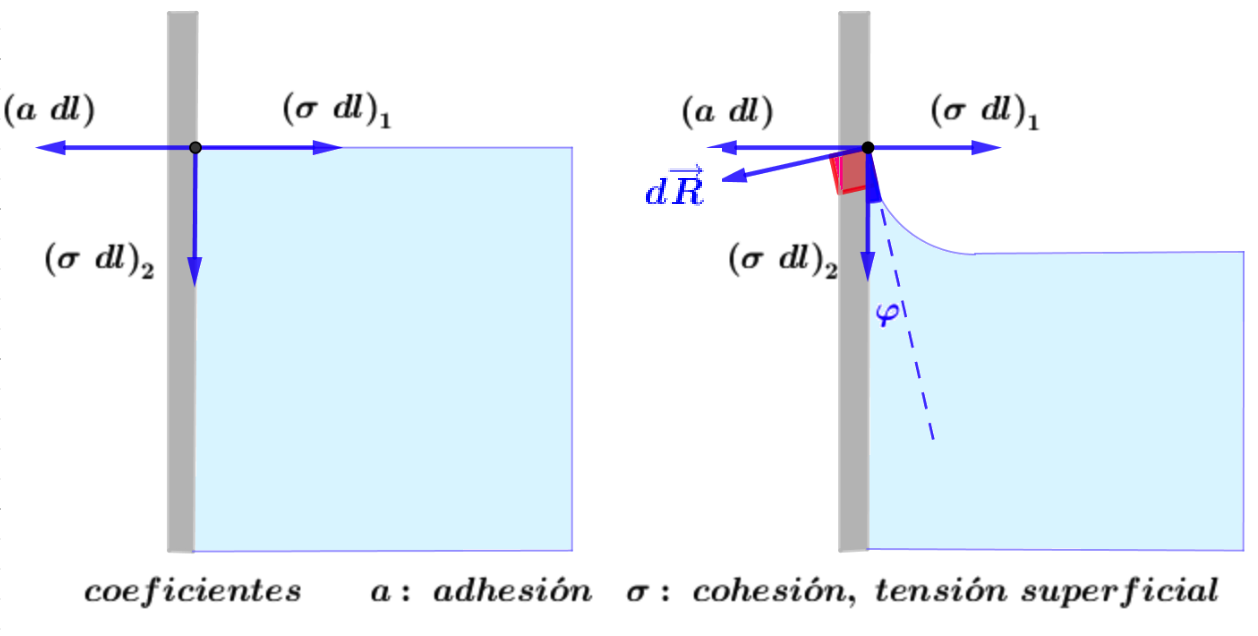
\includegraphics[width=1\textwidth]{imagenes/imagenes08/T08IM05.png}
\end{figure}

Suponemos la superficie del líquido horizontal y estudiamos las fuerzas que aparecen cuando se forma el menisco.

$(\overrightarrow{\sigma \dd l)})_1=\vec i\ \sigma \dd l \sin \varphi - \vec j \ \sigma \dd l \cos \varphi\, \quad$
$(\overrightarrow{\sigma \dd l)})_2=  - \vec j \ \sigma \dd l;$
$\quad (\overrightarrow{a \dd l)})_1=\vec i\ a \dd l$

La resultante, $\dd \vec R$ será: 
$\quad \dd \vec R=\vec i\ (\sigma \sin \varphi - a)\dd l -\vec j \ (1+\cos \varphi) \sigma \dd l$

Ángulo de conjunción: $\quad \tan \varphi=\dfrac {\dd R_y}{\dd R_x}=\dfrac{-\sigma(1+\cos \varphi)}{\sigma \sin \varphi - a}=\dfrac{\sin \varphi}{\cos \varphi}$

Multiplicando en cruz las dos últimas expresiones:

$\sigma \cos^2 \varphi+\sigma \cos \varphi=-\sigma \sin^2 \varphi + a \sin \varphi$

$\sigma=a\sin \varphi - \sigma \cos \varphi$, despejando \small{($\sin \varphi=\sqrt{1-\cos^2 \varphi}$)}\normalsize{:}

\begin{equation}
\cos \varphi=+ \dfrac{a^2-\sigma^2}{a^2+\sigma^2}	
\end{equation}

Expresión que nos da el ángulo de conjunción en función de las propiedades macroscópicas de los cuerpos que actúan.

$\boldsymbol{\sigma}$ es el coeficiente de tensión superficial, depende solo del del líquido. $\boldsymbol{a}$ es el coeficiente de adhesión y depende de la naturaleza del líquido y del recipiente que lo contiene. Un mismo líquido, en distintos recipientes, puede adoptar distintos tipos de meniscos.

Consecuencias:

\vspace{-2mm} \begin{itemize}
\vspace{-2mm} \item $a>\sigma \to \varphi<90^o$, adhesión mayor que cohesión, `el líquido moja el vaso'.	 \textsf{Menisco cóncavo}.
\vspace{-2mm} \item $a<\sigma \to \varphi<90^o$, adhesión menor que cohesión, `el líquido no moja el vaso'. \textsf{Menisco convexo}.	
\end{itemize}

\begin{figure}[H]
	\centering
	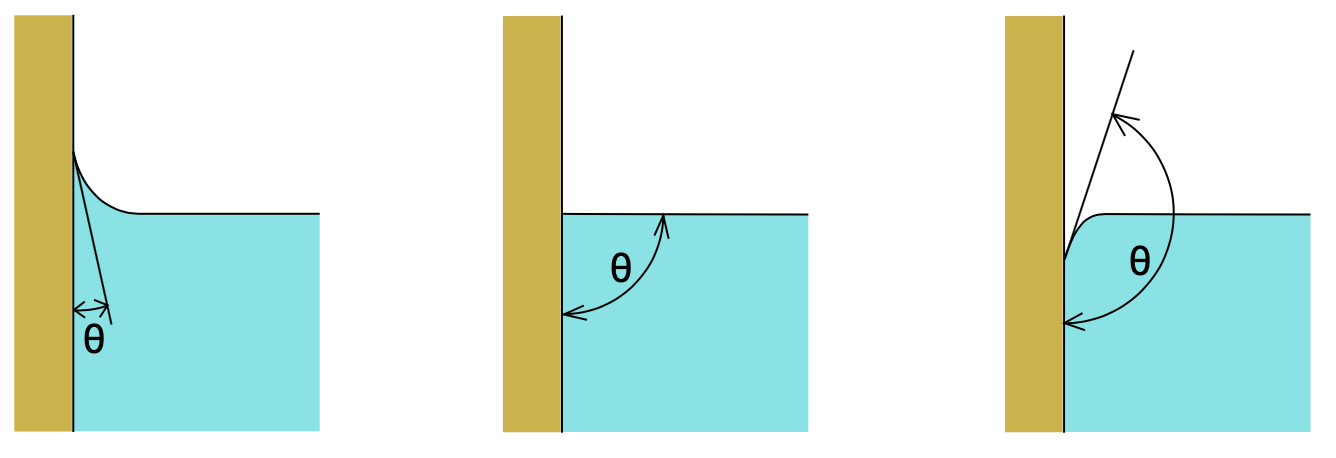
\includegraphics[width=.9\textwidth]{imagenes/imagenes08/T08IM13.png}
\end{figure}

\section{Presión de Laplace}

La existencia de los meniscos tiene como consecuencia el que aparezca una sobrepresión o una depresión sobre toda la masa del líquido, es la conocida como \emph{presión de Laplace.} Para superficies grandes (vaso de agua) es casi imperceptible pero no así para superficies pequeñas (capilar).

Supongamos un elemento de superficie, superficie infinitesimal, de un menisco.

\begin{multicols}{2}
\begin{figure}[H]
	\centering
	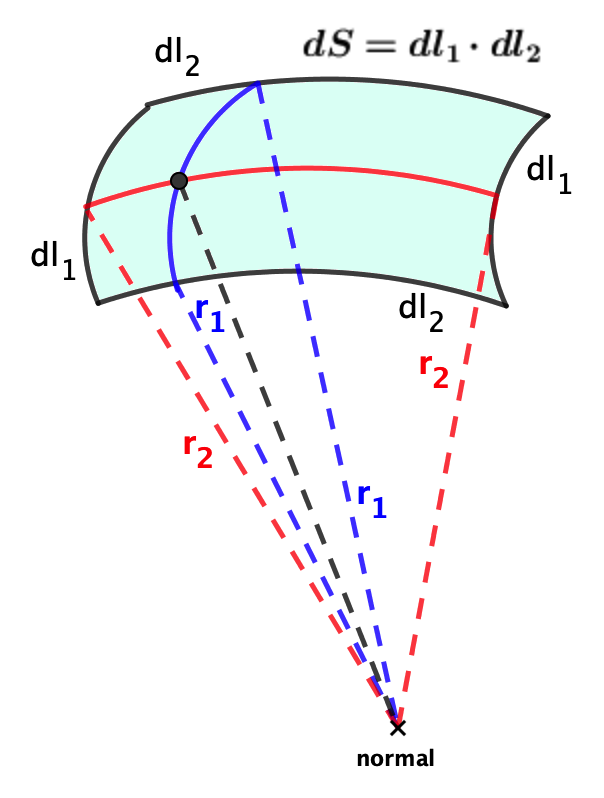
\includegraphics[width=.45\textwidth]{imagenes/imagenes08/T08IM06.png}
\end{figure}
$\quad \quad$ Corte transversal:

\begin{figure}[H]
	\centering
	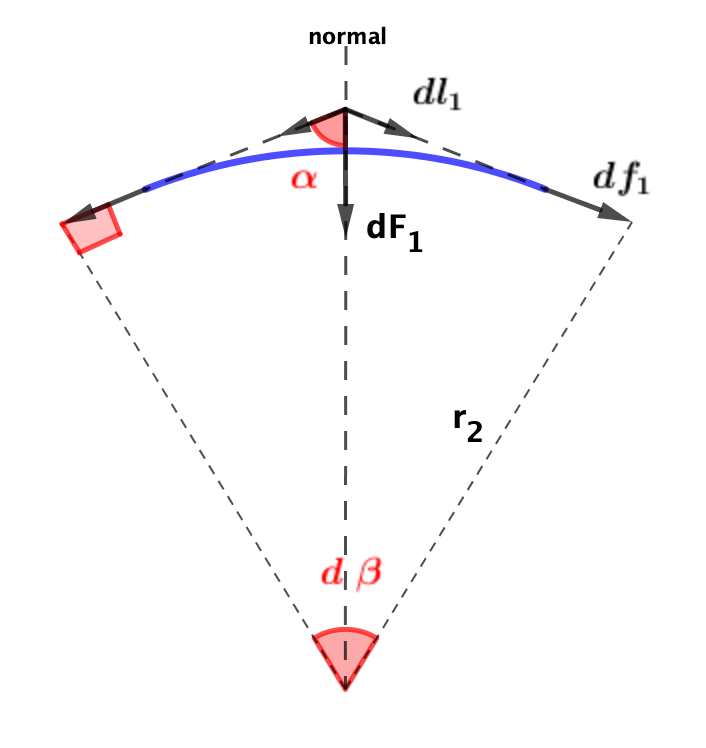
\includegraphics[width=.5\textwidth]{imagenes/imagenes08/T08IM07.png}
\end{figure}
\end{multicols}
Las fuerzas $df_1$ tendrán una resultante $dF_1$ hacia abajo en la dirección normal y que va a influir en todo el líquido.

$\dd F_1=2 \dd f_1 \cos \alpha = 2 \dd f_1 \sin \dfrac{\dd \beta}{2};\ \ \  \qquad \alpha \text{ y } \beta\ $ complementarios.

De matemáticas sabemos que $\sin \dd \beta \approx \dd \beta \qquad  $ 
\textcolor{gris}{
\small{
$\sin x \text{ y } x \ $ son infinitésimos equivalentes: $\ x<1 \to \sin x \approx x$}
\normalsize{.}
} 

$\dd F_1=2\dd f_1 \dfrac {\dd \beta}{2}=\dd f_1\ \dd \beta=\sigma \ \dd l_1 \cdot \dfrac{\dd l_2}{r_2}=\dfrac{\sigma}{r_2}\cdot \dd S \quad $ 
\textcolor{gris}{\small{arco=ángulo x radio}\normalsize{.}}

Análogamente: $\quad \dd F_2= \dfrac{\sigma}{r_1} \cdot \dd S$


La fuerza total: $\quad \dd F=\dd F_1+\dd F_2= \left( \dfrac{\sigma}{r_1}+\dfrac{\sigma}{r_2} \right) \ \dd S$
Como $P=\dfrac {\dd P}{\dd S}$, finalmente tendremos que:

\begin{equation} 
\subrayado{ \ \boldsymbol{ P=	\left( \dfrac{\sigma}{r_1}+\dfrac{\sigma}{r_2} \right) } \ } \qquad \text{ Presión de Laplace.}
\end{equation}

En el caso en que la presión de Laplace no sea despreciable, la \emph{ecuación fundamental de la hidrostática} se escribirá como: $\subrayado{\boldsymbol{P=P_0+\rho g h+ P_L}}$, siendo $P_L$ la presión de Lapalace. Cuando el \textsf{menisco es cóncavo}, $P_L$ representa una \textsf{sobrepresión}; en \textsf{meniscos convexos}, cuando la presión del Laplace no sea despreciable, $P_L$ representará una \textsf{depresión} (la resultante $\dd F$ es hacia arriba, hacia fuera de la superficie del líquido).

Convenio de signos:	
\begin{multicols}{2}
Tomamos los radios como positivos cuando trazados desde el centro de curvatura apuntan al exterior del fluido (meniscos cóncavos - sobrepresión).

Tomamos los radios como negativos cuando trazados desde el centro de curvatura apuntan al interior del fluido (meniscos convexos - depresión).

\begin{figure}[H]
	\centering
	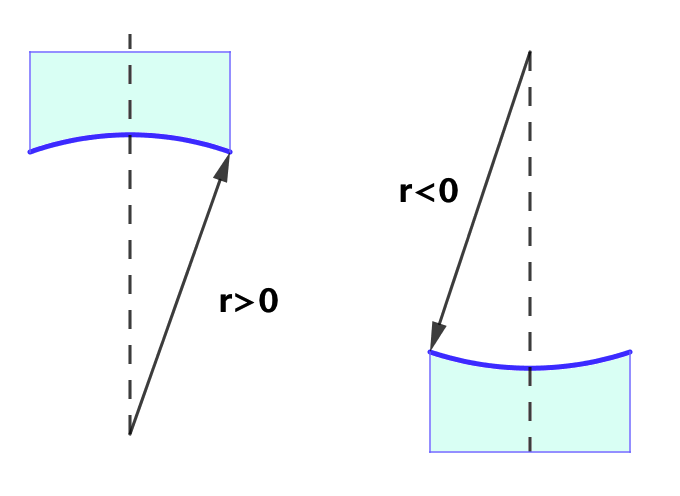
\includegraphics[width=.55\textwidth]{imagenes/imagenes08/T08IM08.png}
\end{figure}
\end{multicols}

\section{Gotas. Ley de Tate}

La forma que tienden a adoptar las masas de líquidos es esférica y se da solo en masas pequeñas debido a la acción del campo gravitatorio terrestre.

La fuerza gravitatoria es proporcional a la masa, es decir, a todo el volumen del cuerpo; la fuerza debida a la tensión superficial es proporcional a la superficie: $\quad F_G \propto V;\quad F_{\sigma} \propto S \ \ \to \quad$
$\dfrac{F_G} {F_{\sigma}}$
$=\dfrac{\frac 4 3 \pi r^3}{4 \pi r^2}=\dfrac 1 3 r$

Para valores grandes de $r$ \textcolor{gris}{los matemáticos dicen: $r>>1$}, la fuerza gravitatoria es mucho mayor que la de tensión superficial, $F_G>>F_\sigma$.  Sabemos, además, que las posiciones de equilibrio exigen una energía potencial mínima (Lejeune Dirichlet \textcolor{gris}{ válido en campos conservativos como el gravitatorio y el electromagnético --Van der Waals--}).

Imaginemos una gota muy grande, gota en posición 1 de la siguiente figura. La energía potencial de una partícula $\dd m$ situada a una altura $y$ es $\dd \mathcal E_p=gy\dd m$. Mientras no exista un mecanismo que lo impida, la gota pasará a la posición 2.

\begin{figure}[H]
	\centering
	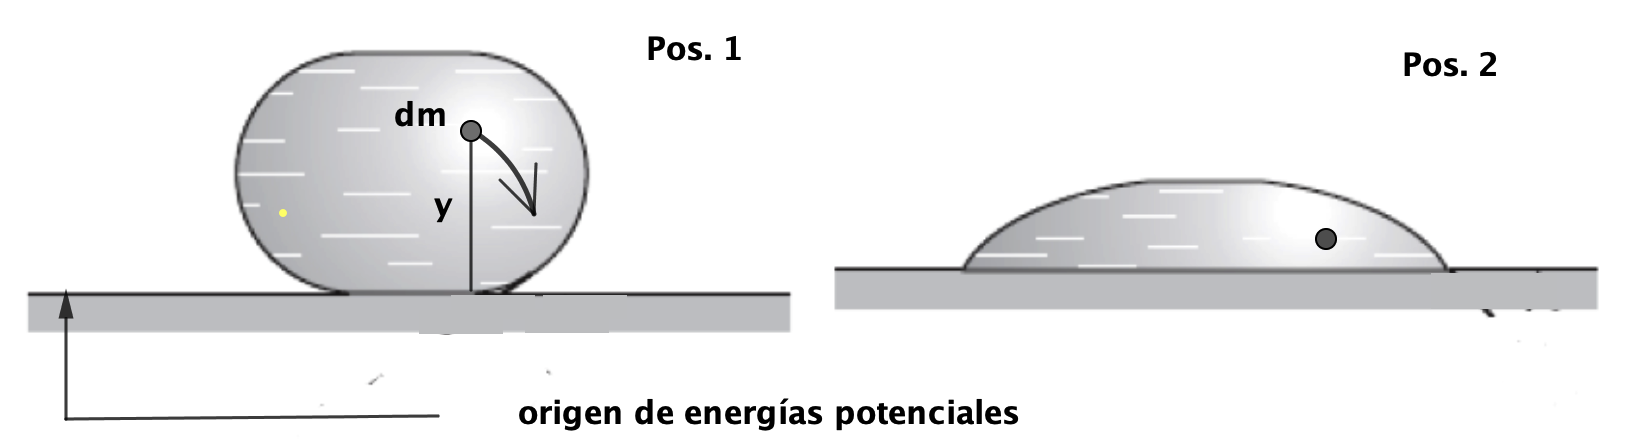
\includegraphics[width=1\textwidth]{imagenes/imagenes08/T08IM09.png}
\end{figure}


Para gotas muy pequeñas, $r \to 0 \Rightarrow \dfrac {F_G}{F_\sigma} \to 0 \Rightarrow F_G<<F_\sigma$ y se adopta la forma esférica de energía potencial mínima.

\textbf{Caída de una gota en un cuentagotas:}


\begin{multicols}{2}
En el momento en que cae la gota, la tensión superficial tiene una resultante hacia arriba que sujeta la gota al cuentagotas hasta que aumentemos la presión en el chupón. Caerá cuando las fuerzas hacia abajo, positivas por convenio, sean mayores que las fuerzas hacia arriba (negativas). En el instante de caer la gota, ambas fuerzas son iguales.

Fuerzas que intervienen:

$+mg;\quad -2\pi r \sigma;\quad -P_0\pi r^2;\quad +P \pi r^2$
\begin{figure}[H]
	\centering
	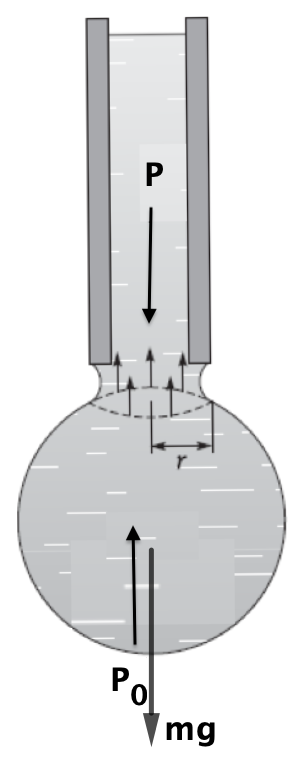
\includegraphics[width=.2\textwidth]{imagenes/imagenes08/T08IM10.png}
\end{figure}	
\end{multicols}

En el instante que cae la gota, la suma total de fuerzas ha de ser cero:

$mg+P\pi r^2=2\pi r \sigma+ P_0\pi r^2$

Por Pascal (ecuación fundamental de la hidrostática): 

$\ P=P_0+\cancelto{0}{P_{\text{altura}}}+P_{Laplace}=P_0+0+\dfrac \sigma r$

\textcolor{gris}{Laplace: $r_1=r;\ \ r_2\to \infty$}

De donde: $\ mg+\pi r^{\cancel{2}} \dfrac{\sigma}{\cancel{r}}+\bcancel{P_0 \pi r^2}=2\pi r \sigma+\bcancel{P_0\pi r^2}$

Se obtiene:

\begin{equation}
\subrayado{\ \boldsymbol{ mg=\pi r \sigma }\ }	 \qquad \text{Ley de TATE}
\end{equation}

La gota se desprende en el mismo momento en que su peso, $mg$ es igual a $\pi r \sigma$ ($r\approx\ $ radio del capilar con el que trabajamos). \textcolor{gris}{Capilar: que tiene un tamaño similar al de una cabello, se dice del tubo muy delgado}.

La ley de Tate es útil para el cálculo de tensiones superficiales y, conocidas éstas y el tamaño del capilar, para el cálculo de la masa de un fluido sin más que contar gotas.

\vspace{3mm}\textbf{Consideraciones:}
\begin{itemize}
\vspace{-2mm}\item Cuando la gota se desprende adopta forma esférica. Para la ley de Laplace a una gota, $r_1=r_2=r\to P_L=2\sigma /r$. La presión $P$ en el interior de la gota es: $\ P=P_0+\dfrac{2\sigma}{r}.\ $ Si la gota es muy pequeña, $P$ es muy grande. Las moléculas que forman la gota están sometidas a una gran presión desde el interior hacia el exterior por lo que las gotas más pequeñas se evaporan más rápidamente.
\vspace{-2mm}\item La gota grande absorbe a la más pequeña:  en la gota grande la presión interna es menor que en la gota pequeña, ello trae como consecuencia que se establezca un \emph{gradiente de presiones} desde la mayor presión (gota pequeña) a la menor presión (gota grande) y ésta última acaba absorbiendo a la gota pequeña.
\end{itemize}

\begin{figure}[H]
	\centering
	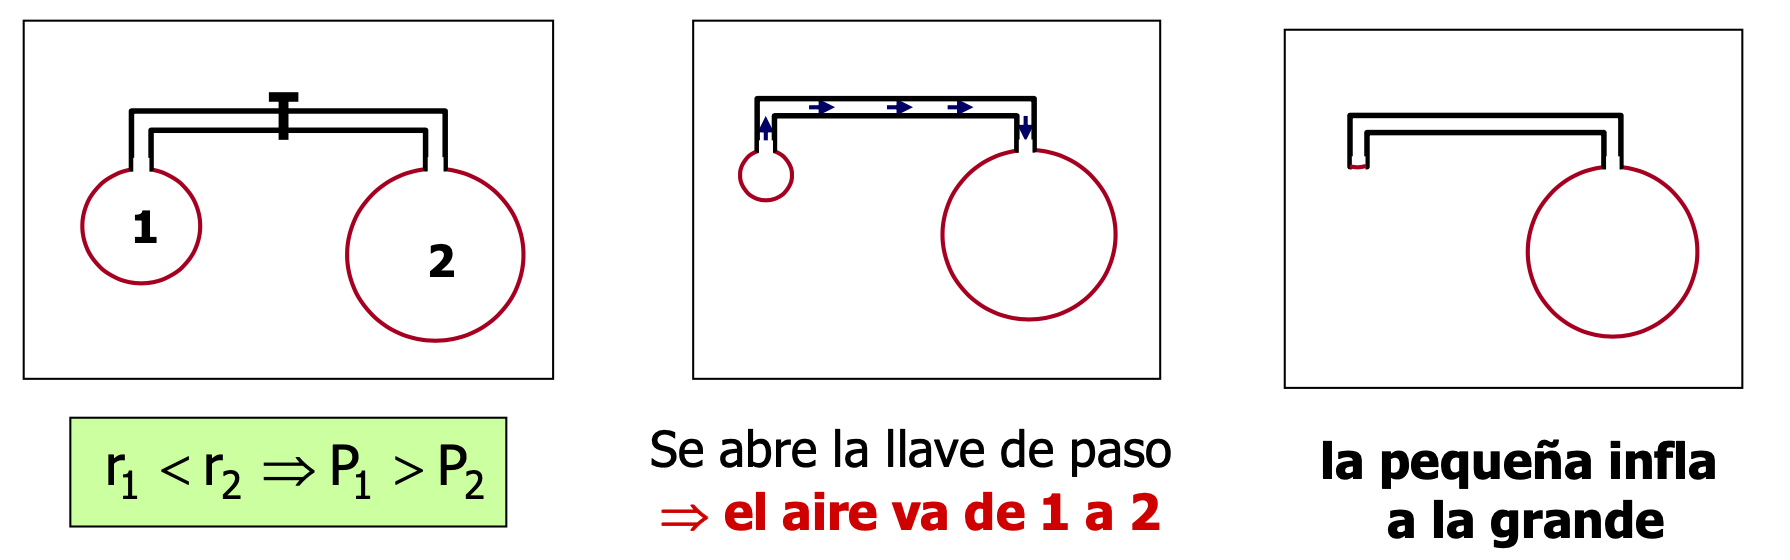
\includegraphics[width=1\textwidth]{imagenes/imagenes08/T08IM18.png}
\end{figure}


\subsection{Pompa de jabón.}

En la superficie $a$, que es convexa respecto a la masa del líquido, la fuerza debida a la presión de Laplace apunta hacia afuera del líquido. La superficie $b$ es cóncava respecto de la masa de fluido y, según Laplace, la fuerza irá hacia el interior de la masa de líquido.
\begin{multicols}{2}
$P=P_0+2\pi \ \dfrac \sigma r+2\pi \ \dfrac \sigma r$

$\quad$

$P=P_0+2\pi \ \dfrac {4\sigma} r$

$\quad$

También explica esta fórmula el efecto de que la gota más grande \emph{chupe} a la más pequeña. A mayor radio, menor presión.
\begin{figure}[H]
	\centering
	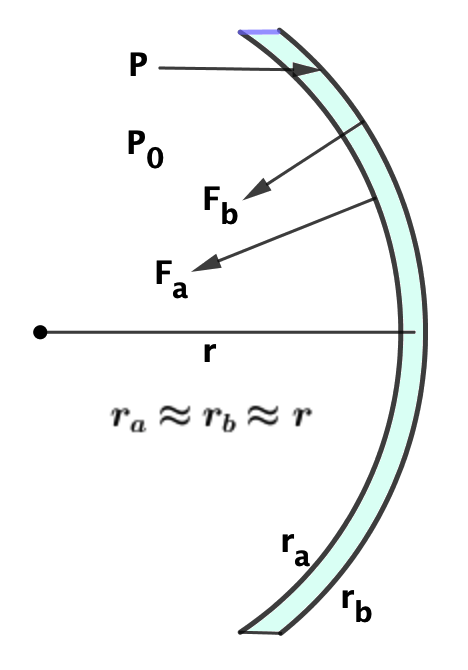
\includegraphics[width=.3\textwidth]{imagenes/imagenes08/T08IM11.png}
\end{figure}
\end{multicols}

\section{Capilaridad. Ley de Jurin}

Supongamos que tenemos un fluido en reposo en un recipiente en el que introducimos un tubo estrecho y abierto.

\begin{multicols}{2}
$\quad$

Se observa el fenómeno que aparece en la figura. \textcolor{gris}{Imagen tomada de Wikipedia.}\footnote{\footnotesize{De MesserWoland - own work created in Inkscape, based on the graphics by Daniel Stiefelmaier, CC BY-SA 3.0, https://commons.wikimedia.org/w/index.php?curid=1353236}\normalsize{.}}

Cuando el tubo es los suficientemente estrecho, \emph{capilar}, el fluido asciende (desciende) por él respecto del nivel del fluido que hay fuera. 

\begin{figure}[H]
	\centering
	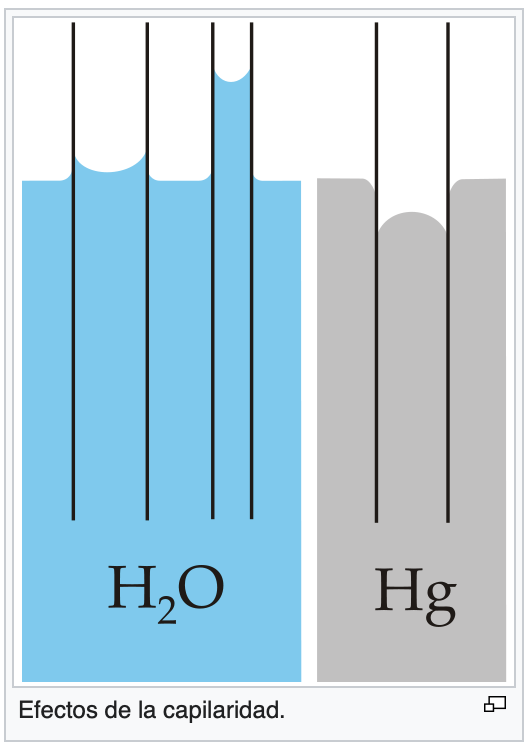
\includegraphics[width=.25\textwidth]{imagenes/imagenes08/T08IM12.png}
\end{figure}

\end{multicols}
En los líquidos que mojan el vaso (meniscos cóncavos), el líquido asciende; en los que no mojan el vaso 8meniscos convexos), el líquido desciende.

\begin{multicols}{2}
Condiciones de equilibrio del fluído en el capilar:

$P_0=P_0`\rho g h-2\dfrac {2\sigma}r$

La presión de la curvatura de Laplace, según el criterio de signos establecido, es negativa.

La presión a nivel del líquido externo en el interior del capilar también es $P_0$ por hidrostática, estamos s al misma altura ($h=0$) y la presión se reparte por igual.


\begin{figure}[H]
	\centering
	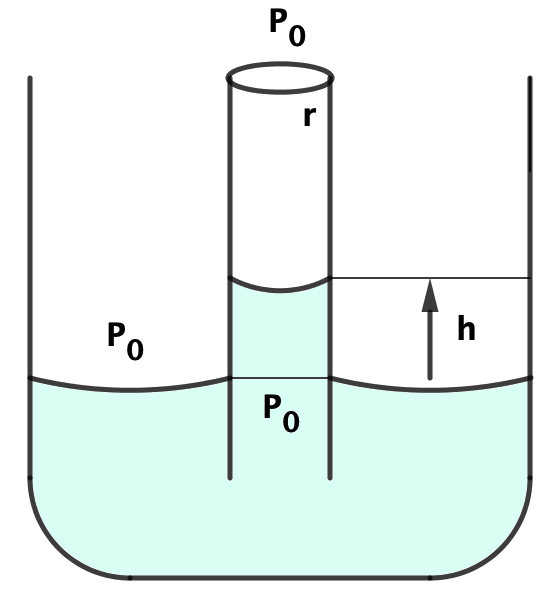
\includegraphics[width=.5\textwidth]{imagenes/imagenes08/T08IM14.png}
\end{figure}	
\end{multicols}

\begin{multicols}{2}
Luego: $\ \rho g h = \dfrac {2\sigma}r$

Como: $\ R=r\cos \phi $,

$\rho g h=\dfrac{2\sigma \cos \varphi}R$
	\begin{figure}[H]
	\centering
	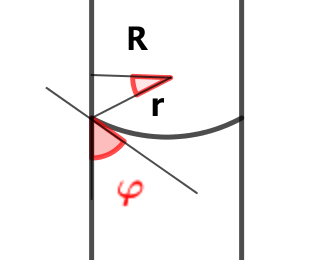
\includegraphics[width=.3\textwidth]{imagenes/imagenes08/T08IM15.png}
\end{figure}
\end{multicols}

\begin{equation}
\subrayado{ \ \boldsymbol{h=\dfrac{2\sigma \cos \varphi}{\rho g R}}	\ } \quad \text{Ley de Jurin}
\end{equation}

Si $R\to 0 \  \rightarrow \ h\to \infty.\ $ Cuanto más pequeño es el capilar, mayor es la altura alcanzada.

Para un capilar $R$ dado, los ascensos y descensos capilares son directamente proporcionales a la tensión superficial del líquido y al coseno del ángulo de conjunción e inversamente proporcionales a la densidad del líquido.

\subsection{Capilaridad en láminas paralelas.}

\begin{multicols}{2}
La altura alcanzada por un líquido entre dos láminas paralelas es la mitad que la que alcanzaría en un tubo cuyo diámetro fuese la mitad de la distancia que separa las láminas.

La fuerza por unidad de longitud, $\sigma \cos \varphi$, actúa sobre los dos lados, $2l$. Esta fuerza se equilibra con el peso del paralelepípedo de fluído $2 r l \cdot h$.
	\begin{figure}[H]
	\centering
	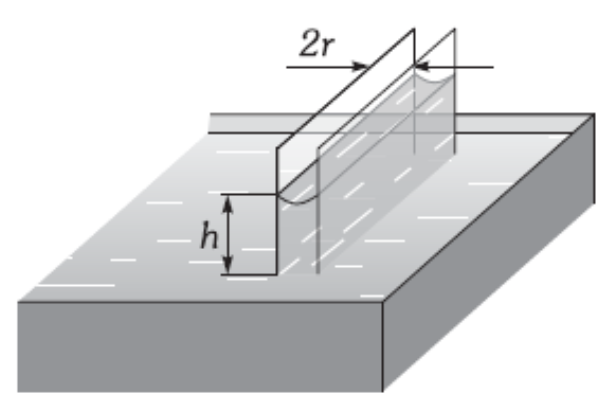
\includegraphics[width=.55\textwidth]{imagenes/imagenes08/T08IM17.png}
\end{figure}
\end{multicols}

\vspace{-4mm} %************************
$$2l\ \sigma \cos \varphi=2rlh\ \rho g \quad \to \quad h=\dfrac{\sigma \cos \varphi}{r\rho g}$$ 

\subsection{Estalagmómetro.}
El estalagmómetro es un aparato de medida de la tensión superficial. Consta de un depósito conectado a un tubo capilar por el que se dejan caer gotas que se pesan. 

 Está ideado de manera que cuando el líquido salga al exterior lo haga en forma de gotas regulares. La zona ancha, tiene un volumen fijo, V, cuando el líquido está comprendido entre las marcas $A$ y $B$.

 
\begin{multicols}{2}
$M=\rho \ V$, para $n$ gotas:

Cada gota, $\ m=\dfrac {\rho\ V}{n}$

Con otro líquido:

$M'=\rho'\ V \to m'=\dfrac {\rho'\ V}{n'}$

Sus pesos:

$mg=\dfrac {\rho\ V}{n}g; \ m'g=\dfrac {\rho'\ V}{n'}g$

De la ley de Tate: 

$\ \dfrac {\rho\ V}{n} g=\pi r \sigma; \ \ \dfrac {\rho'\ V}{n'} g=\pi r \sigma'$ 

\begin{figure}[H]
	\centering
	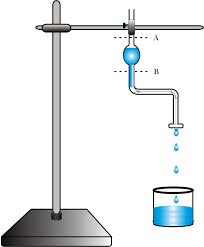
\includegraphics[width=.4\textwidth]{imagenes/imagenes08/T08IM16.png}
\end{figure}	
\end{multicols}
Dividiendo ambas expresiones:$\quad \dfrac{\rho/n}{\rho'/n}=\dfrac \sigma {\sigma'}$

Suponiendo $\sigma'$ conocida, determinamos la tensión superficial del otro líquido $\sigma$ sin más que contar gotas:

$$\boldsymbol{ \sigma\ = \ \sigma' \ \dfrac{\rho'\ n'}{\rho\ n} }$$

\section{Problemas}
\begin{prob}
\begin{multicols}{2}
	Una masa de líquido está girando con velocidad angular $\omega$ constante alrededor del eje vertical que pasa por el centro del recipiente cilíndrico que la contiene. Demuéstrese que la variación de la presión en la dirección radial está dada por $\displaystyle \dv{P}{r}=\rho \omega^2 r$.
\begin{figure}[H]
	\centering
	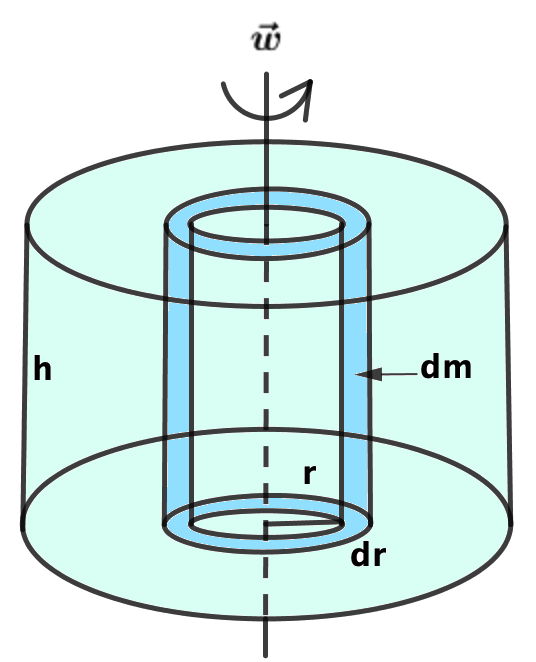
\includegraphics[width=.35\textwidth]{imagenes/imagenes08/T08IM20.png}
\end{figure}
\end{multicols}

\vspace{-4mm} %*********************************
Llamando $P_c$ a la presión en el eje de rotación ($r=0$) y llamando $P$ a la presión a $r$ metros del eje, demuéstrese que: $\ P=P_C+\frac 1 2 \rho \omega^2 r^2$.
\end{prob}


La fuerza normal a que se encuentra sometido el elemento de masa $\dd m$, de espesor $\dd r$ y situado a $r$ metros del eje es:

$\dd F= \dd m a = \dd m \dfrac {v^2}{r}=\dd m \omega^2 r$

Dividiendo por $\dd V \to  \dfrac{\dd F}{\dd V}=\rho \omega^2 r$, con $\rho=\dd m / \dd V$.

Como $V=\pi r^2 h \to \dd V= 2 \pi r h \dd r=S_L \dd r$, con esto,

$\dfrac {\dd F}{\dd V}=\dfrac{\dd F}{S_L \ \dd r}=\dfrac{\dd P}{\dd r}$, con $\dd P=\dfrac{\dd F}{S_L}$

Por lo que, efectivamente: $\ \dfrac{\dd P}{\dd r}=\rho \omega^2 r$

Por ortra parte: $\ \displaystyle \dd P = \rho \omega^2 r \dd r \to \int_{P_c}^P=\int_{0}^r \rho \omega^2 r$, 

de donde: $\ P=P_c+\frac 1 2 \rho \omega^2 r^2$ 

\begin{prob}
Se tiene una suspensión de gotas esféricas de aceite en una mezcla hidroalcoholica de igual densidad ($0.92$). Calcúlese es trabajo realizado por $200$ de estas gotitas al juntarse para formar una sola gota. La tensión superficial del aceite es de $33 \ \mathrm{dinas/cm}$, en el sistema CGS y el diámetro de cada gotita es de $0.2\ \mathrm{mm}$.
\end{prob}

$\dd W = \sigma \dd S \to \ W=\sigma \Delta S=\sigma (4\pi R^2 -n\  4\pi r^2)$, siendo $r$ el radio de las gotitas, $R$ el de la gota grande y $n$ el número de gotitas que formarán la gota.

Falta averiguar $R$, el tamaño de la gota final. Como se conserva la masa de aceite:

$\rho \frac 4 3 \pi R^3= n\ \rho \frac 4 3 \pi r^3 \to \ R=r\ n^{1/3}$

Luego: $W=\sigma \ 4\pi [\ (rn^{1/3})^2-nr^2 \ ]$

$\sigma:\ \ 1 \ \mathrm{dina}=10^{-5}\ \mathrm{N};\ \ 1\ \mathrm{cm} = 10^{-2}\ \mathrm{m} \to \ 33 \ \mathrm{dinas/cm} = \dfrac {33\cdot 10^{-5}}{10^{-2}}=0.033 \ \mathrm{N/m}; \quad r=10^{-4} \ \mathrm{m}; \quad n=200$

Con los datos del problema: $\ \ W=-0.161 \mathrm{J}$, negativo, el campo de fuerza de la tensión superficial realiza el trabajo, la formación de la gota grande es espontánea, no requiere que se realice trabajo exterior.

\begin{prob}
Una gota esférica de radio $3\ \mathrm{mm}$ se divide en dos gotas iguales. Calcula el tamaño de las gotas resultantes y el trabajo que hay que realizar contra la fuerza de la tensión superficial	para dividir la gota grande. La tensión superficie¡al del aceite es $0.47\ \mathrm{J\ m}^{-2}$.
\end{prob}

Como en el problema anterior, $\rho \frac 4 3 \pi R^3 = 2\cdot \frac 4 3 \pi r^3 \to \ r=R\ 2^{-1/3}=2.4\ \mathrm{mm}$

$W=\sigma \Delta S = 4 \pi \sigma (2\cdot r^2-R^2)=14\ \mu \mathrm{J}$


\begin{prob}
\small{Se introduce un capilar de vidrio de $1,0 \ \mathrm{mm}$ de diámetro hasta el fondo de un vaso de agua de $15 \ \mathrm{cm}$ de profundidad y se sopla hasta formar burbujas de aire. a) Determina el exceso de presión del aire respecto a la presión atmosférica en el interior de las burbujas, suponiendo que éstas tienen el mismo diámetro que el capilar. b) Calcula lo que asciende o desciende el agua por el capilar respecto a la superficie del agua cuando se deja de soplar. Supón que el ángulo de contacto del agua con la superficie de vidrio es aproximadamente $0^o$. c) Si se sustituye el agua por glicerina, ?`habrá que soplar con mayor o menor fuerza para formar las burbujas? d) ?es mayor o menor el nivel de la glicerina respecto al agua en el capilar cuando se deja de soplar? Supón que el ángulo de contacto de la glicerina con la superficie de vidrio también es aproximadamente $0^o$. Datos: $\sigma_{agua}=72.8 \ \mathrm{m\ N/m}$, $\sigma_{glicerina}=63.1 \ \mathrm{m\ N/m}$, $\rho_{glicerina}=1.26  \times 10^3 \ \mathrm{kg}/\mathrm{m}^3$	}\normalsize{.}
\end{prob}


---a) El exceso de presión en el interior de las burbujas será:

$P=P_0+\rho g h + \dfrac {2\sigma}{R} \to P-P_0=\rho g h + \dfrac {2\sigma}{R}$, con los datos del problema: $P=1760\ \mathrm{Pa}$

--- b) La altura a la que sube el agua por el capilar es:

$h=\dfrac{2\sigma \cos \varphi}{\rho g R}$, con los datos del problema: $h=0.030 \ \mathrm{m}$

--- c) Si cambiamos por glicerina, el exceso de presión será:

$ P'-P_0=\rho' g h + \dfrac {2\sigma'}{R}$, con los datos del problema: $P'=2100\ \mathrm{Pa}$

--- d) La altura a la que sube la glicerina es:

$h'=\dfrac{2\sigma' \cos \varphi'}{\rho' g R}$, con los datos del problema: $h=0.020\  \mathrm{m}$


\begin{myblock}{Fuerzas intermoleculares. Cohesión.}

\vspace{2mm} Las moléculas de los líquidos no oscilan respecto a posiciones fijas, como ocurre en los sólidos, sino que gozan de cierta libertad de movimiento. 

\vspace{2mm} Las distancias entre moléculas son lo suficientemente pequeñas como para que se ejerzan fuerzas atractivas de cohesión entre las moléculas. 

\vspace{2mm} Como resultado de tales fuerzas, el líquido ocupa un volumen determinado, aunque su forma sea la del recipiente que lo contiene. 

\vspace{2mm} En los gases, las fuerzas de cohesión son muy pequeñas porque las distancias intermoleculares son muy grandes, de modo que los gases tiende a ocupar todo el espacio del que dispongan. 

\vspace{2mm} La existencia de fuerzas de cohesión en los líquidos determina la existencia de una superficie libre y de los fenómenos asociados a ella. 


\vspace{2mm} 
\begin{multicols}{2}
Las fuerzas intermoleculares son de naturaleza electromagnética (\emph{fuerzas de Van der Waals}). Aunque las moléculas sean eléctricamente neutras, cuando dos moléculas se encuentran separadas una distancia suficientemente pequeña, sus distribuciones de carga se alternan, lo que da lugar a la aparición de una fuerza neta, atractiva o repulsiva, entre ambas. 

\begin{figure}[H]
	\centering
	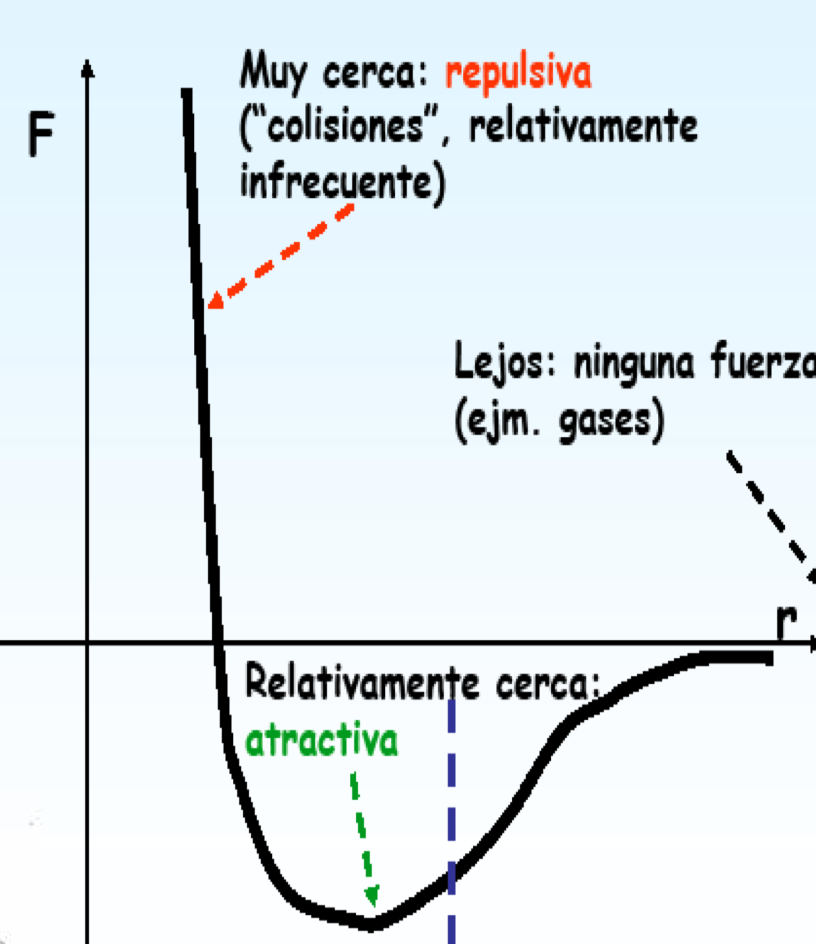
\includegraphics[width=.45\textwidth]{imagenes/imagenes08/T08IM21.png}
\end{figure}
\end{multicols}

\vspace{2mm} La intensidad de las fuerzas intermoleculares varía con la distancia. 

\vspace{2mm} La fuerza repulsiva intermolecular es la responsable de la impenetrabilidad de la materia (de que una molécula pueda atravesar a otra). 

\vspace{2mm} En cualquier caso las fuerzas intermoleculares son de corto alcance, como máximo algunos radios moleculares, 

\vspace{2mm} El efecto de las fuerzas de cohesión sólo es perceptible a una distancia $r$, que llamaremos radio de acción molecular, que es del orden de $10 \ \textup{\r{A}}$. 
\footnote{http://www.ugr.es/~esteban/earth/apuntesbasesfisicas/tr3.pdf}
	
\end{myblock}















